
\begin{frame}
    \frametitle{The FEniCS challenge!}
    Consider steady flow around a cylinder driven by a pressure difference at the left and right boundaries:
    \begin{figure}
    \begin{center}
        \only<1>{
        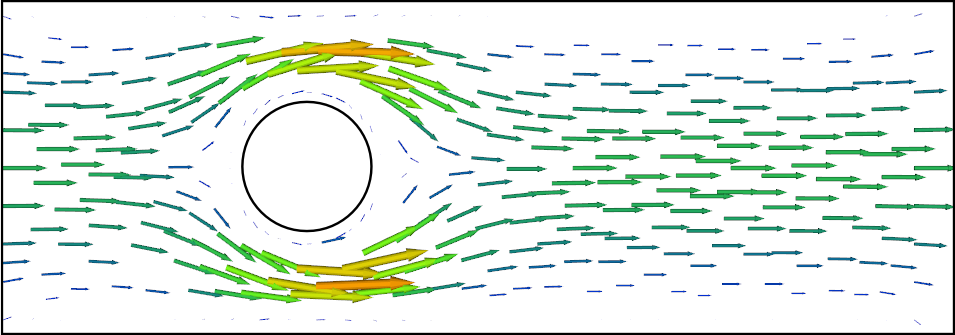
\includegraphics[width=\textwidth]{png/flow_around_cylinder}
        }
        \only<2>{
        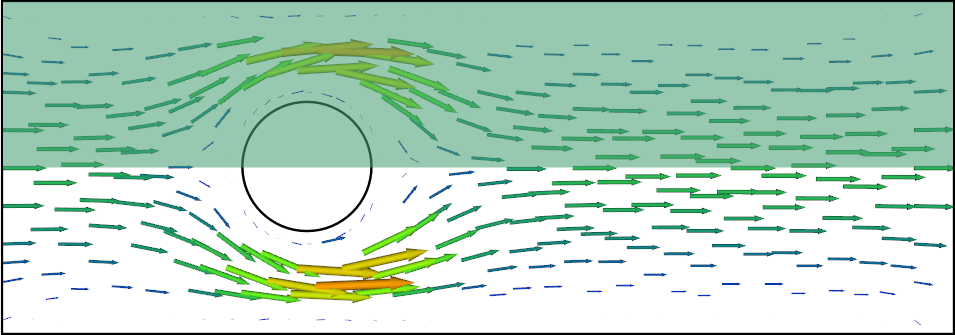
\includegraphics[width=\textwidth]{png/flow_around_cylinder_sponge_area}
        }
    \end{center}
    \end{figure}
    \onslide<2>{
        \begin{itemize}
            \item Imagine you can place sponges in the top half (light green) area of the domain.
            \item How would you place the sponges in order to minimise dissipation of the flow into heat?
        \end{itemize}
    }
\end{frame}

\begin{frame}
    \frametitle{The FEniCS challenge!}

    \begin{equation*}
        \min_{u, f} \int_\Omega \left<\nabla u, \nabla u\right> \dx + \alpha \int_\Omega \left<f, f\right>\dx
    \end{equation*}
    subject to:
    \begin{equation*}
        \begin{aligned}
            - \nu \Delta u + \nabla u \cdot u - \nabla p & = -fu  \quad && \textrm{in } \Omega, \\
            \textrm{div}(u) & = 0 \quad && \textrm{in } \Omega, \\
    \end{aligned}
    \end{equation*}
    with:
        \begin{itemize}
            \item $u$ the velocity,
            \item $p$ the  pressure,
            \item $f$ the control function.
            \item $\nu = 1$ the viscosity,
            \item $\alpha$ the regularisation parameter,
        \end{itemize}
    The boundary conditions are:
        \begin{itemize}
            \item $p = 1$ on the left,
            \item $p = 0$ on the right,
            \item $u = (0,0)$ on the top and bottom and circle.
        \end{itemize}


\end{frame}

\begin{frame}
    \frametitle{The FEniCS challenge!}
    \framesubtitle{Domain}

    \begin{figure}
    \begin{center}
        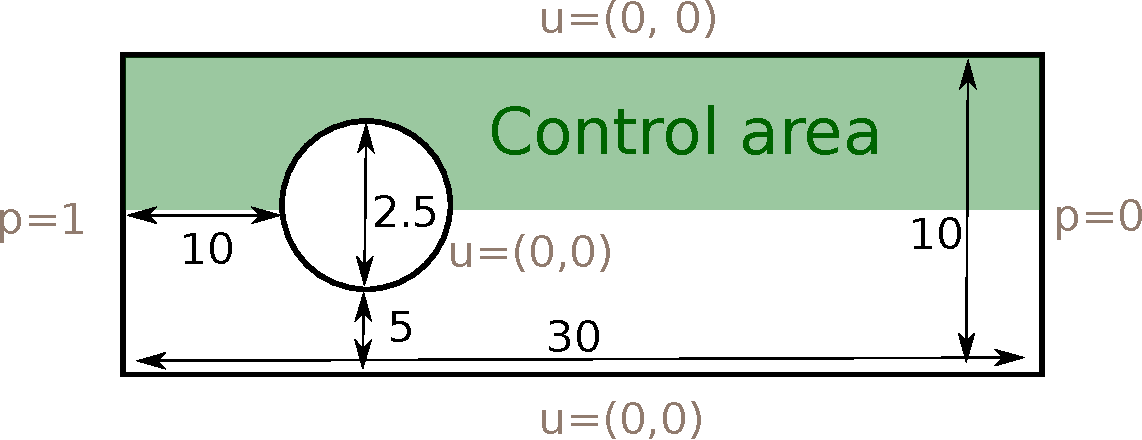
\includegraphics[width=\textwidth]{pdf/optimisation_challenge_domain}
    \end{center}
    \end{figure}

    (Or rather, put the circle with center (10.0, 5.0) and radius 2.5)

    \begin{enumerate}
        \item Write a new program and generate a mesh with the above domain.
    \end{enumerate}

\end{frame}


\begin{frame}
    \frametitle{The FEniCS challenge!}
    \framesubtitle{Navier-Stokes solver}

    The variational formulation of the Navier-Stokes equations is: Find $u, p \in V \times Q$ such that:
    \begin{equation*}
        \begin{aligned}
            \int_\Omega \nu \nabla u \cdot \nabla v + (\nabla u \cdot u + fu) \cdot v +  p \, \Div v \dx & = - \int_{\partial \Omega} p_0 v \cdot n \ds, \\
            \int_\Omega \Div u \, q \dx & = 0 \\
    \end{aligned}
    \end{equation*}
    for all $v \in V$ and all $q \in Q$.

    \begin{enumerate}
        \setcounter{enumi}{1}

        \item Create a \emp{MixedFunctionSpace} consisting of
          continuous piecewise quadratic vector fields for the
          velocity and continuous piecewise linears for the pressure.

        \item Solve the Navier-Stokes equation for $f=0$ and the given
          boundary conditions.
    \end{enumerate}

\end{frame}

\begin{frame}[fragile]
    \frametitle{The FEniCS challenge!}
    \framesubtitle{Optimise}

    \begin{enumerate}
        \setcounter{enumi}{2}
        \item Import \emp{dolfin-adjoint} and define the control parameter and
          functional.
        \item Minimise the functional and plot the optimal control.
        \item What is the minimised functional?
    \end{enumerate}

    \begin{block}{Note}
      Multiply the $\int_\Omega fu\cdot v\dx$ term in the variational
      formulation with the indicator function:
      \vspace{-1em}
      \begin{python}
x = SpatialCoordinate(mesh)
chi = conditional(x[1] >= 5, 1, 0)
      \end{python}
      to ensure that the control is only active in the top half of the
      domain.
    \end{block}

\end{frame}
